\documentclass[a4paper, 12pt]{article}
\usepackage[latin1]{inputenc}
\usepackage[english]{babel}
\usepackage[T1]{fontenc}
\setcounter{section}{0}
\setcounter{figure}{0}
\usepackage{graphicx}
\usepackage{float}
\usepackage{amsmath}
\usepackage{amsfonts}
\usepackage{amsthm}
\usepackage{newlfont}
\usepackage{gensymb}
\usepackage{listliketab}
\usepackage{footnote}

\usepackage{subfig}

\usepackage[dvipsnames]{xcolor}

\usepackage{fancyhdr}
\usepackage{inria}
\usepackage{enumitem}
\setlist[itemize]{noitemsep, leftmargin=10pt}
\usepackage{amssymb}
\usepackage{listings}
\usepackage{hyperref} 
\usepackage{lipsum}
\usepackage[framed,numbered,autolinebreaks,useliterate]{mcode}
\lstset{language=Matlab, basicstyle=\scriptsize\ttfamily, frame=single}


\colorlet{punct}{red!60!black}
\definecolor{background}{HTML}{EEEEEE}
\definecolor{delim}{RGB}{20,105,176}
\colorlet{numb}{magenta!60!black}



\lstdefinelanguage{json}{
    basicstyle=\normalfont\ttfamily,
    numbersep=8pt,
    showstringspaces=false,
    breaklines=true,
    frame=lines,
    backgroundcolor=\color{background},
    literate=
     *{0}{{{\color{numb}0}}}{1}
      {1}{{{\color{numb}1}}}{1}
      {2}{{{\color{numb}2}}}{1}
      {3}{{{\color{numb}3}}}{1}
      {4}{{{\color{numb}4}}}{1}
      {5}{{{\color{numb}5}}}{1}
      {6}{{{\color{numb}6}}}{1}
      {7}{{{\color{numb}7}}}{1}
      {8}{{{\color{numb}8}}}{1}
      {9}{{{\color{numb}9}}}{1}
      {:}{{{\color{punct}{:}}}}{1}
      {,}{{{\color{punct}{,}}}}{1}
      {\{}{{{\color{delim}{\{}}}}{1}
      {\}}{{{\color{delim}{\}}}}}{1}
      {[}{{{\color{delim}{[}}}}{1}
      {]}{{{\color{delim}{]}}}}{1},
}

%\lstloadlanguages{Matlab}
%\usepackage{rotating}

%-------------------------------
% DEFINIZIONE DEGLI ENVIRONMENT
%-------------------------------

\newtheorem{obs}{Osservazione}[section]
\newenvironment{oss}
    {\begin{obs}\begin{normalfont}}
    {\hfill $\square \!\!\!\!\checkmark$ \end{normalfont}\end{obs}}

\newtheorem{pro}{Problema}[section]
\newenvironment{prob}
    {\begin{pro}\begin{normalfont}}
    {\hfill $\spadesuit$ \end{normalfont}\end{pro}}

\newtheorem{teor}{Teorema}[section]
\newenvironment{teorema}
    {\begin{teor}\textit }
    {\hfill  \end{teor}}

\newtheorem{defn}{Definizione}[section]
\newenvironment{de}
    {\begin{defn}\begin{normalfont}}
    {\hfill $\clubsuit$ \end{normalfont}\end{defn}}

%-----------------------------
% CONFIGURAZIONE DELLA PAGINA
%-----------------------------

\hfuzz2pt % Don't bother to report over-full boxes if over-edge is < 2pt

\fancypagestyle{plain}{
\fancyhead{}\renewcommand{\headrulewidth}{0pt} } \pagestyle{fancy}
%\renewcommand{\chaptermark}[1]{\markboth{\small CAP. \thechapter \textit{ #1}} {} }
\renewcommand{\sectionmark}[1]{\markright{\small  \thesection \textit{ #1}} {} }
\voffset=-20pt    % distanza tra il limite superiore del foglio e l'intestazione
\headsep=40pt     % distanza  l'intestazione ed il testo del corpo
\hoffset=0 pt     % misura equivalente al margine sinistro
\textheight=620pt % altezza del corpo del testo
\textwidth=435pt  % larghezza del corpo del testo
\footskip=40pt    % distanza tra il testo del corpo ed il pie' di pagina
\fancyhead{}      % cancella qualsiasi impostazione per l'intestazione
\fancyfoot{}      % cancella qualsiasi impostazione per il pie' di pagina
\headwidth=435pt  % larghezza del'intestazione e del pie' di pagina
\fancyhead[R]{}%{\rightmark} \fancyfoot[L]{\leftmark}
\fancyfoot[R]{}%{\thepage}
\renewcommand{\headrulewidth}{0.3pt}   % spessore della linea dell'intestazione
\renewcommand{\footrulewidth}{0.3pt}   % spessore della linea del pi�di pagina

\numberwithin{equation}{section}
\renewcommand{\theequation}{\thesection.\arabic{equation}}
%--------------------------
% MODIFICARE DA QUI IN POI
%--------------------------

\begin{document}
\titoloTesi{Privacy Preserving Contact Tracing}
\corso{Hack the Crisis [NL]}  
%\corso{Lorenzo Mazzeo, Francesco Prinari, Jacopo Diamanti, Giovanni Balestrieri}  
\anno{4 april 2020}

\baselineskip=25pt

\intestazione

%------------------------------------------------
% INTRODUZIONE E RINGRAZIAMENTI (NON MODIFICARE)
%------------------------------------------------

\fancypagestyle{plain}{
\fancyhead\renewcommand{\headrulewidth}{0pt} } \pagestyle{fancy}
%\renewcommand{\chaptermark}[1]{\markboth{\small Cap. \thechapter \textit{ #1}} {} }
\renewcommand{\sectionmark}[1]{\markright{\small  \S \thesection \textit{ #1}} {} }
\voffset=-20pt                         % distanza tra il limite superiore del foglio e l'intestazione
\headsep=40pt                          % distanza  l'intestazione ed il testo del corpo
\hoffset=0pt                           % misura equivalente al margine sinistro
\textheight=620pt                      % altezza del corpo del testo
\textwidth=435pt                       % larghezza del corpo del testo
\footskip=40pt                         % distanza tra il testo del corpo ed il pie' di pagina
\fancyhead{}                           % cancella qualsiasi impostazione per l'intestazione
\fancyfoot{}                           % cancella qualsiasi impostazione per il pie' di pagina
\headwidth=435pt                       % larghezza del'intestazione e del pie' di pagina
\fancyhead[R]{\rightmark} \fancyfoot[L]{\leftmark}
\fancyfoot[R]{\thepage}
\renewcommand{\headrulewidth}{0.3pt}   % spessore della linea dell'intestazione
\renewcommand{\footrulewidth}{0.3pt}   % spessore della linea del pié di pagina

\pagenumbering{Roman} \tableofcontents
\newpage

\pagenumbering{arabic}

\fancyhead[R]{Introduzione} \fancyfoot[L]{Introduzione}
\fancyfoot[R]{\thepage}


\fancyhf{} %elimina header/footer vecchi


\fancyhead[R]{\rightmark} \fancyhead[L]{\leftmark}
\fancyfoot[R]{\thepage}


%-----------------------
% DEFINIZIONE VARIABILI
%-----------------------

\newcommand{\figura}{figura}

%---------------------
% INCLUSIONE CAPITOLI
%---------------------

{\color{PineGreen}\section{Summary}}

This document is a report written during the \textbf{Hack the Crisis NL} online hacakthon\cite{bib1}. We propose a system for secure and privacy-preserving contact tracing. Providing a technological foundation to help slow the spread of the SARS-CoV-2 virus.\\

Goals:
\begin{itemize}
\item Take advantage of existing implemented solutions to brake transmission chains and control the spread of the disease,
\item Avoid Identity Driven solutions. We don't ask citizens to provide their identity,
\item Inform the user if there is an infection in their contact chain,
\item Automate the process of inferring the list of possible users that might have been exposed to an infected person in the 14 days preceding the test
\end{itemize} 

The system aims to minimise single point of failure, privacy and security risks for citizens and communities and to guarantee data protection.

To achieve this goal, we use mobile applications to continuously track anonymous users (we do not ask them to provide email,name, surname or ID numbers) and ask them to report symptoms, if they are using Individual Protection Devices or protective clothing when they go out. The information is encrypted and stored in an ummutable decentralized digital ledger called Tangle. 
Whenever a patient is diagnosed, verified Health Departments, testing laboratories or Drive In testing facilities send his universal unique identifier (uuid) of the the application to the Tangle and flags it as an infected uuid. \\
\\
As soon as a new infected uuid is published on the ledger a computer (no server is required, works with a personal computer as well) performs the contact tracing task and uuids at risk are broadcasted.\\
If the application sees its uuid on the Tangle, the user is notified of the risk so that he/she can then take preventive actions such as self-isolating or wearing a ffp3 mask.

\begin{figure}[H]
	\begin{center}
	    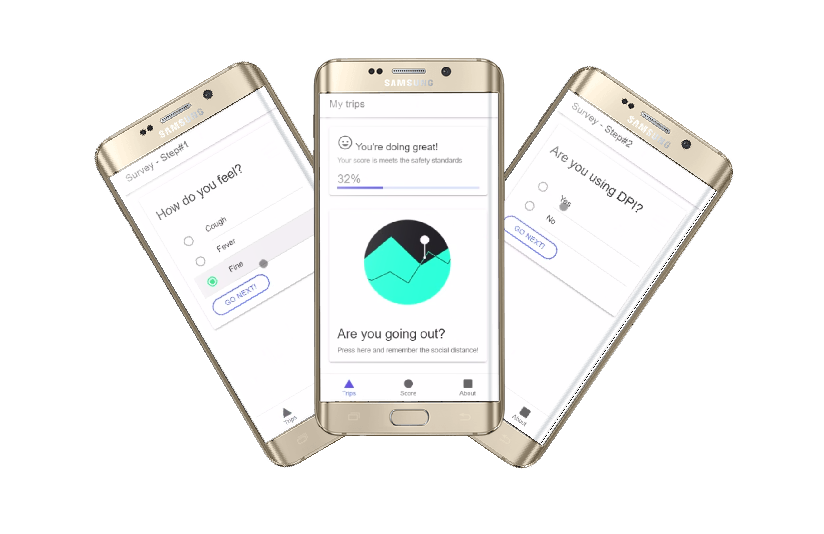
\includegraphics[scale=0.9]{imgs/phones_1.pdf}
 		\caption{Self-report information about the symptoms}
 		\label{fig:hi_low}
	\end{center}
\end{figure}


%pseudo-random ID representing the user and also record pseudo-random IDs observed from
%smartphones in close proximity. Whenever a patient is diagnosed, he or she can upload
%some anonymous data from their phone to a central server. This step should only be done
%with the approval of a health authority and the consent of the individual. Before, no data is
%communicated to any entity. Other instances of the app can use the anonymous data from
%the server to locally compute whether the app's user was in physical proximity and
%potentially infected by an infected person and to inform the user of the risk. Additionally, the
%system enables users to voluntarily provide information to epidemiologists, in a
%privacy-preserving manner, to enable studies of the evolution of disease and to assist in
%finding better policies to prevent further infections

Additionally, the system enables users to voluntarily provide information to epidemiologists to enable studies of the evolution of disease in the region of interest and to assist in finding better policies to prevent further infections.
\\
We provide a description about security aspects, privacy properties, architecture and the provided features. 
\\
The code is available on Github and released under the GNU GPL v3 license so that further protection mechanisms can be added if weaknesses are identified and additional features can be added by the community.


%
%\begin{equation}
%    \chi = \begin{bmatrix}
%        x \\ y \\ \theta
%     \end{bmatrix}\qquad \qquad
%Y = \begin{bmatrix}
%        y \\ \theta
%     \end{bmatrix}\qquad \qquad
%U = \omega
%\end{equation}
%in which:
%\begin{itemize}
%	\item x, y: Linear positions of the center of the camera respectively along the x and y axes
%	\item $\theta$: Angular position of the center of the camera along the z-axis
%	\item $\omega$: Angular velocity along the z-axis which represents the input of the system
%	\item v: velocity vector of the center of gravity of the robot. Assumed to be constant
%\end{itemize}
%The following subsections present dynamic models considered in during the simulation and design of the controller
%{\color{PineGreen}\subsection{Simplified system}}
%Discrete system with sampling time $\delta_{T}$
%\begin{align}
%    x(k+1) ={} & x(k) + \vert v \vert \delta_{T} cos(\theta(k))
%\\
%	y(k+1) ={} & y(k) + \vert v \vert \delta_{T} sin(\theta(k))\label{eq:pointMass}
%\\
%	\theta(k+1) = {} &  \theta(k)+\omega(k) \delta_{T} =  \theta(k)+u(k) \delta_{T} 
%\end{align}
%
%{\color{PineGreen}\subsection{Perturbed Simplified system}}
%In a real world scenario, Toutilo's description can be affected by unmodeled dynamics which force the robot to steer towards an unknown direction even if no angular velocity command is executed. This phenomenon can be approximated by an uncertain constant angular velocity drift $\omega_{D}$. In addition, when driving over low-traction, deformable terrains or even steep hills, external forces have to be considered in order to achieve acceptable results. An approximation of these forces can be introduced in the system by considering a linear velocity component $v_{y}$.
%\\
%\begin{itemize}
%	\item $\omega_{D}$ : Angular drift along the z-axis. [ Uncertainty ]
%	\item $v_{y}$ : linear velocity vector resulting from an external force acting on the center of mass of the robotic platform [ external forces ]
%\end{itemize}
%
%The resulting discrete system is described by:
%\begin{equation}
%    x(k+1) = x(k) + [\vert v \vert  cos(\theta(k)) - \vert v_{y} \vert sin(\theta(k))]\delta_{T}
%\end{equation}
%\begin{equation}
%    y(k+1) = y(k) + [\vert v \vert  sin(\theta(k)) + \vert v_{y} \vert cos(\theta(k))]\delta_{T}
%\end{equation}	
%\begin{equation}
%   	\theta(k+1) = \theta(k)+(u(k)+\omega_D) \delta_{T} 
%\end{equation}
%
%{\color{PineGreen}\subsection{Perturbed and constrained Simplified system}\label{subsec:pertconstrained}}
%
%It is worth noting that the low level controller of Toutilo presents several non-linearities that have to be taken into account during the design of the control system. A dead zone of $ \pm 5 mrad/s$ associated to the control input $\omega$.\newline
%\\
%Let us introduce two new inputs:
%\begin{itemize}
%	\item $u_S = sat(u(\cdot), max, min)$ : is a saturation function of the control input
%	\item $u_D = deadZ(u(\cdot), max, min)$ : is a dead zone applied to the control input
%\end{itemize}
%The new system is described by:
%\begin{equation}
%    x(k+1) = x(k) + [\vert v \vert  cos(\theta(k)) - \vert v_{y} \vert sin(\theta(k))]\delta_{T}
%\end{equation}
%\begin{equation}
%    y(k+1) = y(k) + [\vert v \vert  sin(\theta(k)) + \vert v_{y} \vert cos(\theta(k))]\delta_{T}
%\end{equation}	
%\begin{equation}
%   	\theta(k+1) = \theta(k)+(u_S(k)+\omega_D) \delta_{T} 
%\end{equation}
%\begin{equation}
%   	u_S = sat(u_D(k), max_{sat}, min_{sat})
%\end{equation}
%\begin{equation}
%   	u_D = deadZ(u(k), max_{deadZ}, min_{deadZ})
%\end{equation}
%
%{\color{PineGreen}\subsection{Differential Drive system}}
%
%
%{\color{PineGreen}\subsection{Perturbed and constrained Differential Drive system}}
{\color{PineGreen}\section{Contact Tracing}}

Contact tracing is a strategy for breaking transmission chains and controlling the spread of the disease. Contact tracing is most effective as a means of containing flareups. Applying this strategy can prevent exponential growth in new cases, protect health-care systems and potentially save lives.
\\
{\color{PineGreen}\subsection{Description}}
It involves identifying infected persons, finding those with whom the infected person may have been in close contact while infectious, locating and testing these close contacts. If a close contact is found to be infected, the disease-investigation process starts again.
\\
It is extremely important to identify asymptomatic or paucisymptomatic because these cases can transmit the virus. This investigation helps public-health departments to draw lines of transmission accurately. Contact tracing could help find those people and ask them to self-isolate.\\

{\color{PineGreen}\subsection{Current base approaches}}

The algorithm for the management of contacts of probable or confirmed COVID-19 cases issued by the 
European Center for Disease prevention and control is described below:

\begin{figure}[H]
	\begin{center}
	    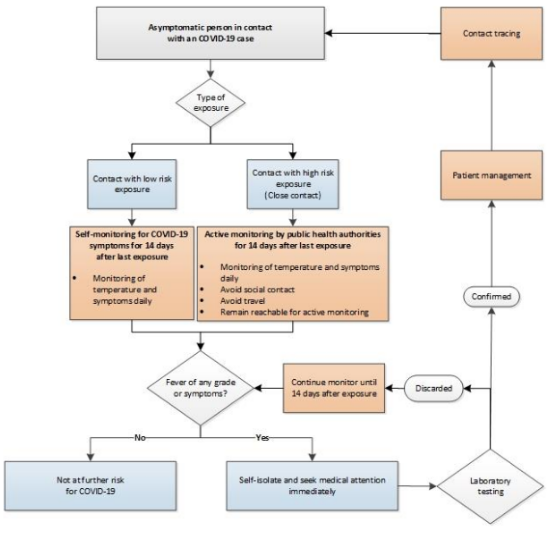
\includegraphics[scale=0.7]{imgs/algo_eu.png}
 		\caption{Algorithm for the management of contacts of probable or confirmed COVID-19}
 		\label{fig:algo_eu}
	\end{center}
\end{figure}

During the contact investigation, the IDD makes a distinction between high-risk and low-risk contacts. 

\begin{figure}[H]
	\begin{center}
	    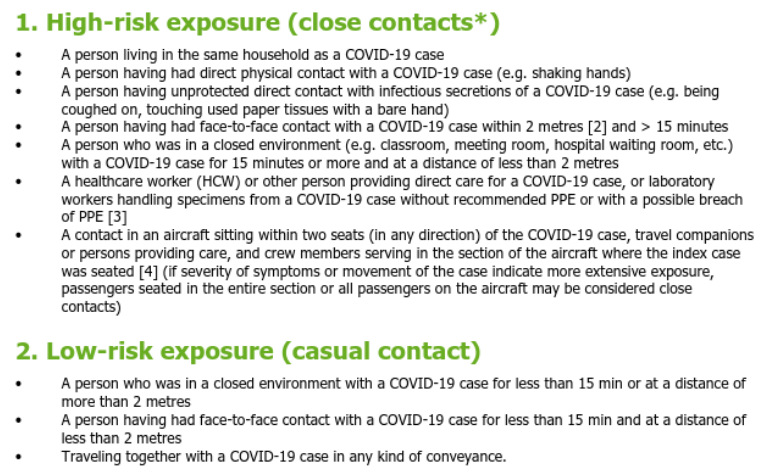
\includegraphics[scale=0.5]{imgs/hi_low.png}
 		\caption{Distinction between high and low-risk contacts}
 		\label{fig:hi_low}
	\end{center}
\end{figure}

Current modes of operation in the Netherlands\cite{bib3} and in Italy are described in the following sub sections.\\
{\color{PineGreen}\subsubsection{The Netherlands}}
If a person tests positive for the coronavirus, the Infectious Disease department (IDD) of the municipal or regional Health Service will be notified. The IDD contacts the patient or another designated contact person and maps out who the patient has been in contact with during the contagious period. From the first day of illness of the patient - the day someone starts to cough or develop symtoms - until the last moment of contact that the patient has had with someone.
\\
{\color{PineGreen}\subsubsection{Italy}}
In Italy, we rely on covid patients' past memories. They ask if they remember who they have been in contact with. If they miss someone, the forgotten citizen will be potentially the next patient 0 and the deadly will loop strike back.

{\color{PineGreen}\section{The race to new methods}}

In this section we quickly discuss the methods used by other countries to improve contact tracing.

{\color{PineGreen}\subsection{Main idea}}

Researchers and technologists all around the world are developing several mobile based solutions that alert users when they have come into contact with someone with coronavirus. Proximity or location data are used to notify someone who has recently been near to an infected individual, so that they can then take preventive action such as self-isolating.\\
\\
These solutions could safely help transition out of national lockdowns and relax social distancing rules while defending against a second wave of infections. Medical researchers and bioethicists at the University of Oxford found that digital contact tracing had the potential to achieve epidemic control if used by enough people.
\\
{\color{PineGreen}\subsection{Bluetooth based methods}}
One of the most popular formats to emerge have been bluetooth based apps. By taking advantage of th low energy protocol, bluetooth identifiers and signal strength from other nearby phones they keep a record of them for a set period of time. This approach allows both outdoor and indoor tracking and is considered by privacy advocates as the least intrusive form of mobile tracking.
Several solutions have been released under free software or less restrictive open source licences. Other proprietary solutions are spreading as well. 
\\
{\color{PineGreen}\subsection{Gps Alternatives}}

An alternative solution could be GPS location tracking technology. Teams at MIT are exploring this solution (Safe Paths) on top of their bluetooth offering. There is emerging evidence that coronavirus can be transferred via surfaces even after a period of time suggesting it may be better to monitor where someone went rather than with whom they crossed paths.\\
\\
But GPS location data is harder to anonymise and researchers are still looking for ways to better encrypt data.
\\
{\color{PineGreen}\subsection{Related problems}}
The main concerns are related to privacy and the possibility of data leakage by the involved actors in the logic.\\
Related information:
\begin{itemize}
\item Beijing appeared to share citizen's data with the police.
\item South Korea has broadcast the personal information of infected people when alerting others who may have been exposed to them.
\item In Israel, security services are controversially tapping data collected by the country's mobile phone operators.
\end{itemize}

{\color{PineGreen}\subsection{Indentified proprietary solutions}}
\begin{itemize}
\item \textit{Pan-European Privacy-Preserving Proximity Tracing}\cite{bib4} claims to interrupt new chains of SARS-CoV-2 transmission rapidly and effectively by informing potentially exposed people. They enable tracing of infection chains across national borders. 
\item \textit{Covid19 Contact Alert} Combining NFC and Blockchain technology to monitor contact moments and alert people. German technology company MYNXG\cite{bib5} introduces a blockchain technology to enable privacy compliant pandemic tracking on regular smartphones. People can download a special app on their smartphone and use any existing NFC to connect their smartphone to the MYNXG blockchain. This technology provides privacy when monitoring individual movements or alerting people if there is an infection in their contact chain. 
\end{itemize}



{\color{PineGreen}\section{Our approach}}
It's time to sleep now. 
{\color{PineGreen}\subsection{Time contrained decisions}}

{\color{PineGreen}\subsection{Possibility to include bluetooth}}
{\color{PineGreen}\subsection{Solved problems}}

{\color{PineGreen}\subsection{Related problems}}


{\color{PineGreen}\section{Architecture}}


{\color{PineGreen}\subsubsection{Mobile applications}}
{\color{PineGreen}\subsubsection{RiskAssesor}}
{\color{PineGreen}\subsubsection{Distributed Digital Ledger}}

{\color{PineGreen}\section{The race to new methods}}
%
%{\color{PineGreen}\subsection{Related problems}}
%
%{\color{PineGreen}\subsection{Indentified proprietary solutions}}
%

{\color{PineGreen}\section{Data protection}}

{\color{PineGreen}\section{Scalability}}

{\color{PineGreen}\section{Epidemiological Research}}


% ELENCO DELLE FIGURE (OPZIONALE)
%\addcontentsline{toc}{chapter}{Elenco delle figure}
%\listoffigures


% BIBLIOGRAFIA
\addcontentsline{toc}{chapter}{References}
\begin{thebibliography}{11}

	\bibitem{bib1} Hack the Crisis NL online Hackathon, \emph{``https://www.hackthecrisis.nl/en''}.
	
	\bibitem{bib2} European Centre for Disease Prevention and Control , \emph{``https://www.ecdc.europa.eu/en/publications-data/public-health-management-persons-including-health-care-workers-having-had-contact''}.
	
	\bibitem{bib3} Zo werkt contactonderzoek bij het coronavirus, \emph{``https://www.nu.nl/coronavirus/6035667/zo-werkt-contactonderzoek-bij-het-coronavirus.html''}.
	
	
	\bibitem{bib4} Pan-European Privacy-Preserving Proximity Tracing, \emph{``https://www.pepp-pt.org/''}.
	
	\bibitem{bib5} Covid19 Contact Alert service, \emph{``https://www.mynxg.com/''}.
		
		
\end{thebibliography}

\end{document}
